\section{Evaluation}

\begin{frame}{Evaluation}
  \begin{itemize}
    \item \textbf{Evaluated:} Three implemented graph partitioning algorithms.
          \begin{itemize}
            \item Random
            \item Oblivious
            \item Coordinated
          \end{itemize}
    \item \textbf{Evaluated:} Three implemented PowerGraph abstraction runtimes.
          \begin{itemize}
            \item{Bulk Synchronous}
            \item{Asynchronous}
            \item{Asynchronous Serializable}
          \end{itemize}
    \item \textbf{Not Evaluated:} Performance relative to other similar
          frameworks/languages.
  \end{itemize}
\end{frame}


\subsection{Evaluating 3 Graph Partitioning Methods}

\begin{frame}
  \frametitle{\small{Do Improved V-Cut Methods Reduce Replication on Big Graph
              Datasets?}}
  \centering
  \begin{figure}
    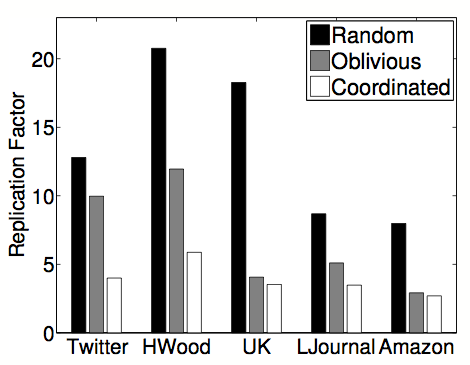
\includegraphics{gonzalez_osdi_2012_figure_7a}
    \caption{\cite[OSDI '12]{gonzalez2012powergraph}}
  \end{figure}
\end{frame}

\begin{frame}
  \frametitle{\small{Do Improved V-Cut Methods Reduce Runtime on Big Graph
              Analysis Tasks?}}
  \centering
  \begin{figure}
    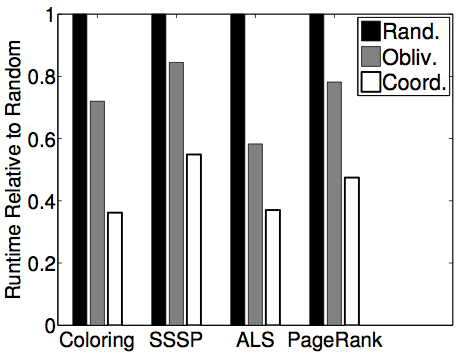
\includegraphics{gonzalez_osdi_2012_figure_7b}
    \caption{\cite[OSDI '12]{gonzalez2012powergraph}}
  \end{figure}
\end{frame}

\begin{frame}
  \frametitle{\small{Do Improved V-Cut Methods Improve Scaling of Replication
              Rates? (Twitter)}}
  \centering
  \begin{figure}
    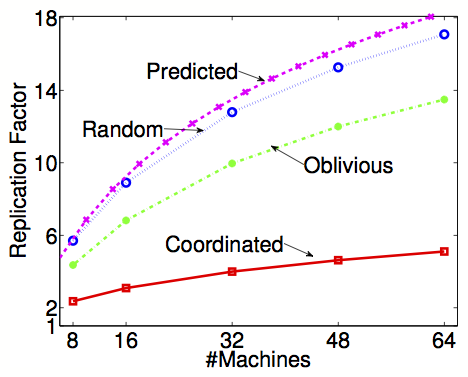
\includegraphics{gonzalez_osdi_2012_figure_8a}
    \caption{\cite[OSDI '12]{gonzalez2012powergraph}}
  \end{figure}
\end{frame}

\begin{frame}
  \frametitle{\small{Do V-Cut Algorithms \textit{Themselves} Scale Well?
              (Twitter)}}
  \centering
  \begin{figure}
    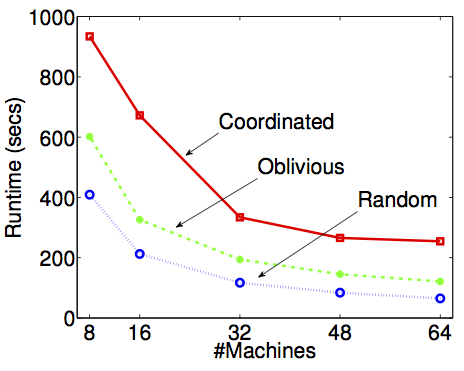
\includegraphics{gonzalez_osdi_2012_figure_8b}
    \caption{\cite[OSDI '12]{gonzalez2012powergraph}}
  \end{figure}
\end{frame}

\begin{frame}
  \textbf{TODO:} Include graphs/charts for your evaluation
\end{frame}
